% Intended LaTeX compiler: pdflatex
\documentclass[bigger]{beamer}
\usepackage[utf8]{inputenc}
\usepackage[T1]{fontenc}
\usepackage{graphicx}
\usepackage{longtable}
\usepackage{wrapfig}
\usepackage{rotating}
\usepackage[normalem]{ulem}
\usepackage{amsmath}
\usepackage{amssymb}
\usepackage{capt-of}
\usepackage{hyperref}
\mode<beamer>{\usetheme{Madrid}}
\mode<beamer>{\usepackage{amsmath}}
\usetheme{default}
\author{Kostas Papadimos}
\date{}
\title{For 16/11}
\hypersetup{
 pdfauthor={Kostas Papadimos},
 pdftitle={For 16/11},
 pdfkeywords={},
 pdfsubject={},
 pdfcreator={Emacs 28.2 (Org mode 9.5.5)}, 
 pdflang={English}}
\begin{document}

\maketitle

\section{1st attempt}
\label{sec:org81ed697}
\begin{frame}[label={sec:org8cdec61}]{Simulation}
\begin{center}
\begin{tabular}{l}
500 \texttimes{} 10\textsuperscript{3} Events for training and Testing\\
Signal parent mass: 10 Gev\\
Background parent mass: 13 Gev\\
Pt Eta Phi coordinates\\
\end{tabular}
\end{center}
\end{frame}

\begin{frame}[label={sec:orgb45f5fe}]{Output}
\begin{center}
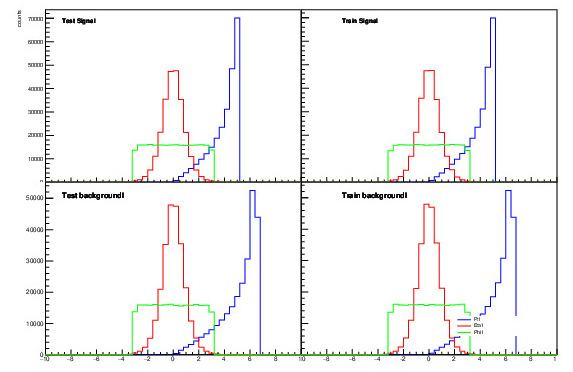
\includegraphics[width=\textwidth]{/home/kpapad/UG_thesis/Thesis/Sim/out/PLots/S10B13_restDataPlot.jpeg}
\end{center}
\end{frame}

\begin{frame}[label={sec:org2190c31}]{Training}
\begin{center}
\begin{tabular}{lr}
\alert{Params} & \alert{Config}\\
max depth & 9\\
sub sample & 0.3\\
n estimators & 1000\\
learning rate & 0.5\\
gamma & 5\\
objective & binary:logistic\\
early stopping rounds & 50\\
eval metric & auc\\
\end{tabular}
\end{center}
\end{frame}

\begin{frame}[label={sec:org8982681}]{Results}
\begin{center}
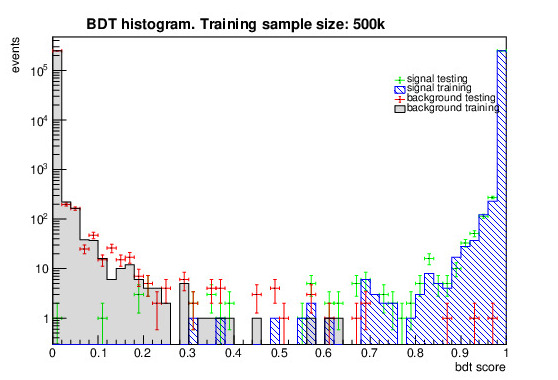
\includegraphics[width=.9\linewidth]{/home/kpapad/UG_thesis/Thesis/Bdt/out/Plots/S10B13_rest500kConf10BDTplot.jpeg}
\end{center}
\end{frame}
\section{2nd attempt}
\label{sec:org1fc0647}
\begin{frame}[label={sec:org9c7b4d6}]{Simulation}
This time, I din't produce new data. I used less data points 200K training events and 200K testing simply bu importing the first 200k events from each data set.
\end{frame}
\begin{frame}[label={sec:orgec47dc0}]{Training}
Same as before 
\end{frame}
\begin{frame}[label={sec:orgb3c392c}]{Results}
\begin{center}
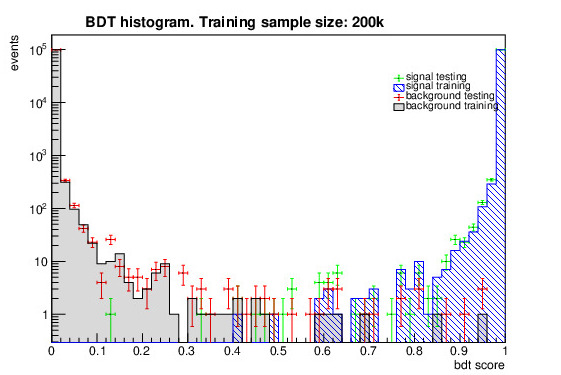
\includegraphics[width=\textwidth]{/home/kpapad/UG_thesis/Thesis/Bdt/out/Plots/S10B13_rest200kConf10BDTplot.jpeg}
\end{center}
\end{frame}
\section{3d attempt}
\label{sec:orgd405665}
\begin{frame}[label={sec:org11d5bf8}]{Simulation}
Instead of generating 1M events and then splitting them in half(for training and testing), I created different sets of 500k events for testing and training,
\begin{center}
\begin{tabular}{l}
500 \texttimes{} 10\textsuperscript{3} Events for training and Testing\\
Signal parent mass: 10 Gev\\
Background parent mass: 13 Gev\\
Pt Eta Phi coordinates\\
\end{tabular}
\end{center}
\end{frame}
\begin{frame}[label={sec:orga234fad}]{Output}
\begin{center}
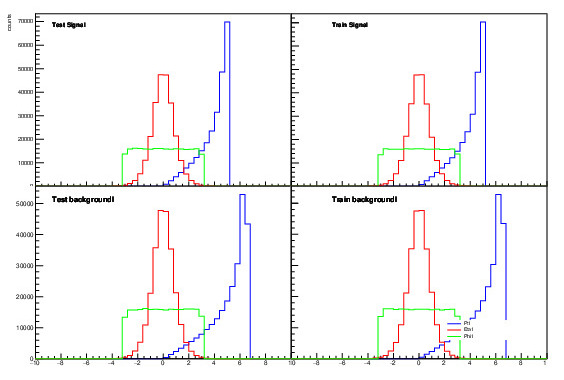
\includegraphics[width=\textwidth]{/home/kpapad/UG_thesis/Thesis/Sim/out/PLots/S10B13_rest2DataPlot.jpeg}
\end{center}
\end{frame}
\begin{frame}[label={sec:orga3c4509}]{Training}
Same as before
\end{frame}
\begin{frame}[label={sec:org868add6}]{Results}
\begin{center}
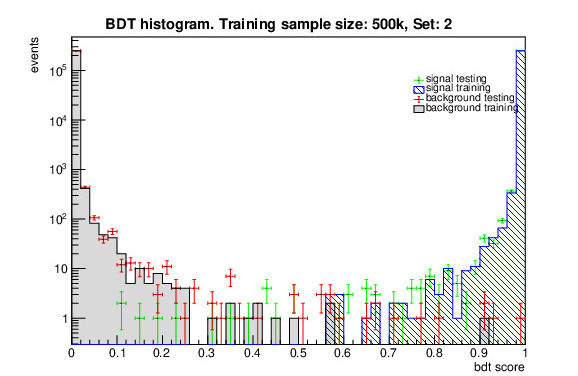
\includegraphics[width=\textwidth]{/home/kpapad/UG_thesis/Thesis/Bdt/out/Plots/S10B13_rest500k_2Conf10BDTplot.jpeg}
\end{center}
\end{frame}
\section{4th attempt}
\label{sec:orgecb1362}
\begin{frame}[label={sec:orgaf56bde}]{Simulation}
This time, I used 3d attempt's data set, and only Pt1 Ph1 Eta1
the settings where the same as ed attempt
\end{frame}
\begin{frame}[label={sec:org44f5b9d}]{Training}
I tried two different training configurations 
\begin{center}
\begin{tabular}{lrr}
\alert{Params} & \alert{Config1} & \alert{Config2}\\
max depth & 9 & 5\\
sub sample & 0.3 & 0.8\\
n estimators & 1000 & 1500\\
learning rate & 0.5 & 0.1\\
gamma & 5 & 0\\
objective & binary:logistic & bnary:logistic\\
early stopping rounds & 50 & 50\\
eval metric & auc & log loss\\
\end{tabular}
\end{center}
\end{frame}
\begin{frame}[label={sec:orgea4b512}]{Results}
\end{frame}
\begin{frame}[label={sec:org212b6ac}]{1st configuration}
\begin{center}
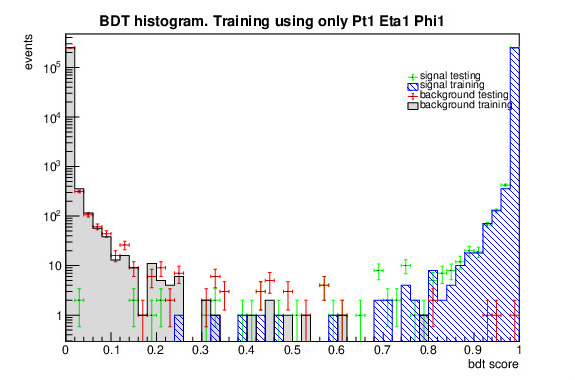
\includegraphics[width=\textwidth]{/home/kpapad/UG_thesis/Thesis/Bdt/out/Plots/S10B13_rest500k_1VecConf10BDTplot.jpeg}
\end{center}
\end{frame}

\begin{frame}[label={sec:org1d7b1ea}]{2nd configuration}
\begin{center}
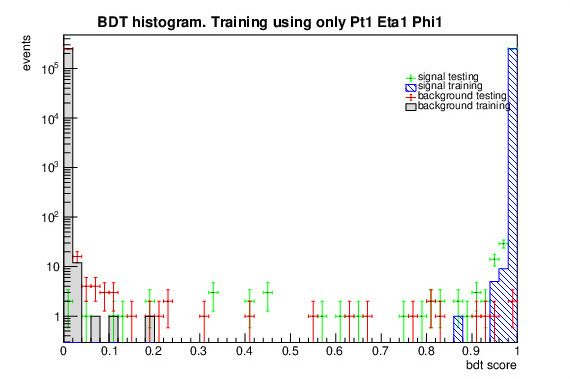
\includegraphics[width=\textwidth]{/home/kpapad/UG_thesis/Thesis/Bdt/out/Plots/S10B13_rest500k_1VecConf9BDTplot.jpeg}
\end{center}
\end{frame}
\end{document}